\chapter{Introduzione}

\section{Il corso in breve...}

\subsection{Cosa si intende per programmazione concorrente?}

La programmazione concorrente nasce con i \fancyglitter{sistemi concorrenti} nell'ambito dei \newfancyglitter{sistemi operativi} con il concetto di \newfancyglitter{processo} (o \newfancyglitter{thread}). 

\dfn{Sistema concorrente}{
  Un sistema concorrente è un sistema \newfancyglitter{software} implementato su una \newfancyglitter{piattaforma hardware} in grado di eseguire \textbf{\newfancyglitter{contemporaneamente}} più attività diverse che condividono \newfancyglitter{risorse comuni}\footnote{Porzioni di memoria centrale, CPU, etc.}. 
}

\nt{Un esempio di sistemi concorrenti sono i \newfancyglitter{sistemi operativi multiprogrammati}.}

\cor{Programma concorrente}{Un programma concorrente è un insieme di \evidence{moduli sequenziali} che possono essere eseguiti in parallelo.}

\subsubsection{Tipi di parallelismo:}

\begin{itemize}
  \item [$\Rightarrow$] \newfancyglitter{Parallelismo reale}: l'esecuzione dei moduli è realmente sovrapposta nel tempo;
  \item [$\Rightarrow$] \newfancyglitter{Parallelismo apparente}: si applica la tecnica d'\fancyglitter{interleaving delle istruzioni}.
\end{itemize}

\nt{In entrambi i casi il termine \fancyglitter{concorrenza} si utilizza come un'astrazione per studiare il parallelismo.
}

\subsubsection{In questo corso si tratterà di:}

\begin{itemize}
  \item Introduzione ai \fancyglitter{principi} della programmazione concorrente;
  \item Analisi dei principali \fancyglitter{costrutti linguistici} per la programmazione concorrente;
  \item Applicazione di questi costrutti a vari problemi di \fancyglitter{sincronizzazione} e \fancyglitter{comunicazione} in programmi concorrenti;
  \item Studio delle \fancyglitter{proprietà di correttezza} dei programmi concorrenti: \newfancyglitter{no deadlock}, \newfancyglitter{no starvation}, etc. 
\end{itemize}

\subsection{Cosa si intende per algoritmo distribuito?}

\dfn{Sistema distribuito}{
  Un sistema distribuito è un sistema composto da \newfancyglitter{più computer} che non condividono la memoria o altre risorse, ma sono connessi da canali di comunicazione\footnote{Debolmente connessi.}.
}

\cor{Algoritmo distribuito}{
  Un algoritmo distribuito è un algoritmo progettato per essere eseguito da un sistema distribuito.
}

\begin{figure}[h]
    \centering
    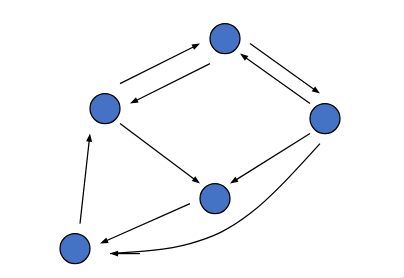
\includegraphics[scale=0.4]{01-IntroduzioneAllaProgrammazioneConcorrente/AlDist.png}
    \caption{Schema di un sistema distribuito}
\end{figure}

\subsubsection{Obiettivi per la parte di corso di algoritmi distribuiti:}

\begin{itemize}
\item Introduzione di modelli formali che permettano l'analisi di \fancyglitter{algoritmi distribuiti di base};
\item Studio della \fancyglitter{correttezza} e delle \fancyglitter{prestazioni} degli algoritmi distribuiti presentati;
\item Analisi di \fancyglitter{algoritmi distribuiti} in presenza di \fancyglitter{malfunzionamenti} (algoritmi fault tolerant).
\end{itemize}

